В ходе выполнения этого этапа я определил требуемую полосу пропускания реального канала связи. Для этого я установил рассчитанные на предыдущем этапе средние значения уровней шумов, рассинхронизации и граничного напряжения.

Затем, изменяя порядковый номер нижней гармоники от нуля и верхней гармоники от максимального значения, я определил граничные значения полосы пропускания, при которых сообщение передается без ошибок для каждого из методов кодирования. Затем определил необходимую ширину полосы пропускания для каждого метода кодирования.

\subsection{NRZ}

\begin{wrapfigure}{l}{0.63\textwidth}
	\centering
	% 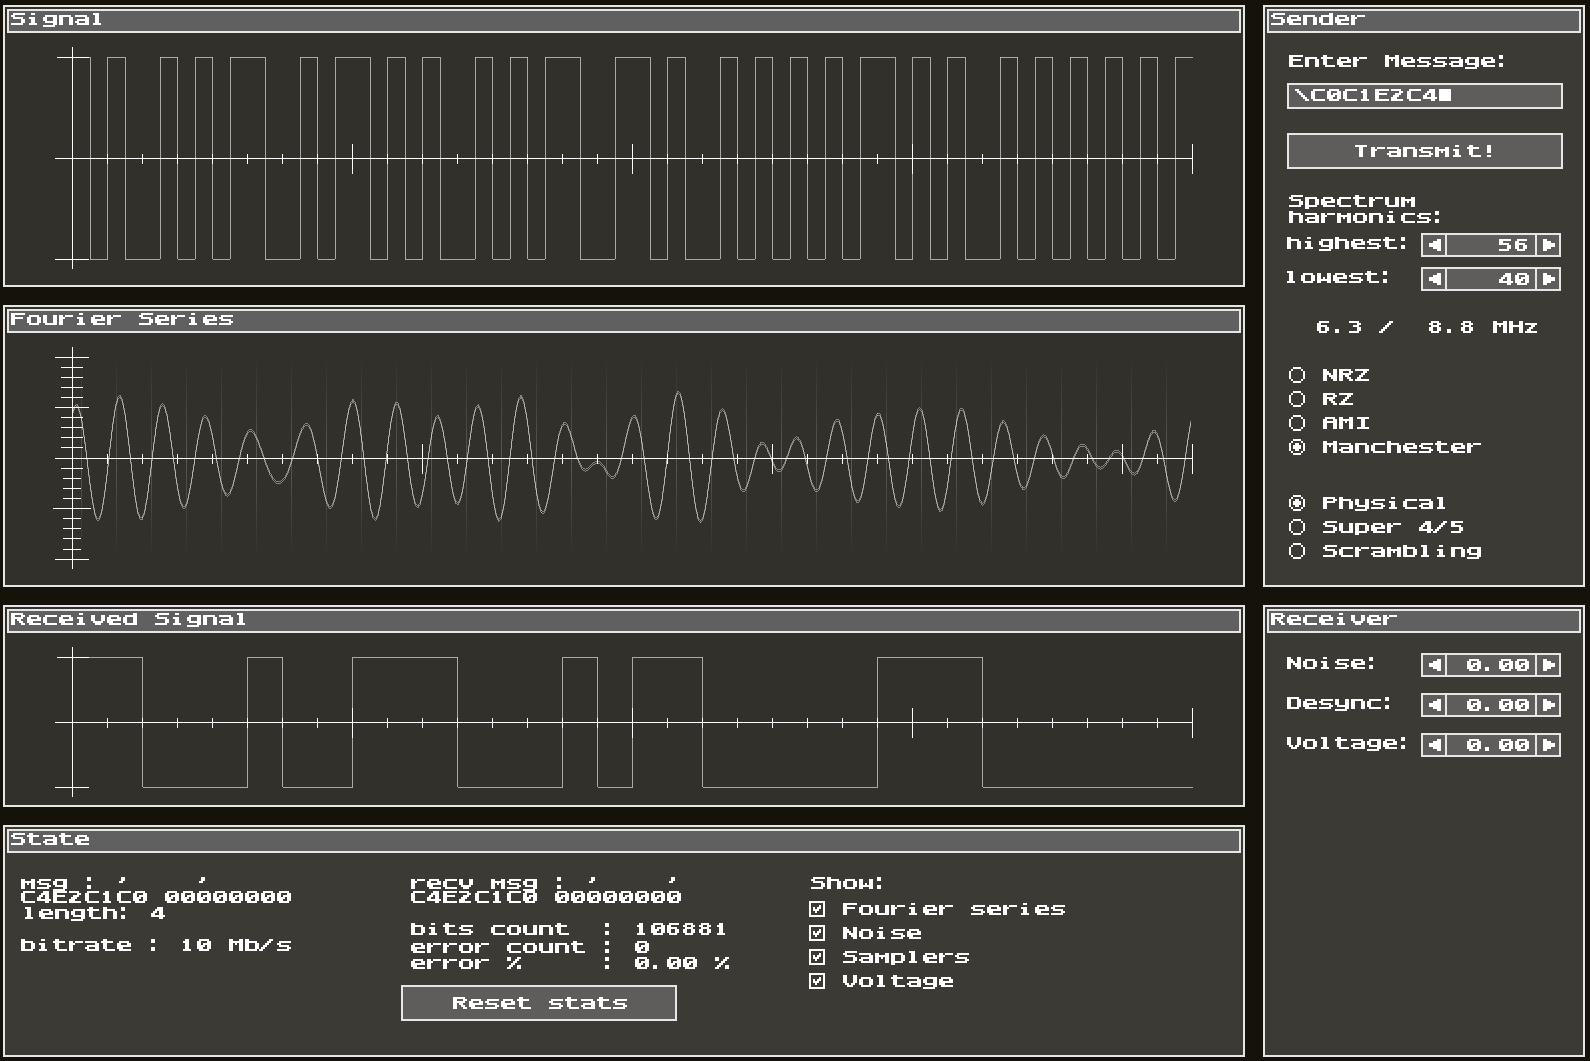
\includegraphics[width=0.95\linewidth]{./data/ideal_m2_min_f.png}
	\cutpic{0.2cm}{11cm}{./data/6_nrz.png.jpg}
	\caption{F =  1.3 - 4.4 Мгц}
    \vspace{-2.1cm}
\end{wrapfigure}

Для метода NRZ требуемая ширина полосы пропускания реального канала связи составила 3.1 МГц.
Для передачи данных без ошибок в условия реального канала связи пришлось увеличить верхнюю границу частот. Ширина полосы пропускания увеличилась с 2.5 МГц до 3.1 МГц (изменилась на +0.6 МГц).

\subsection{RZ}

\begin{wrapfigure}{r}{0.5\textwidth}
	\centering
	% 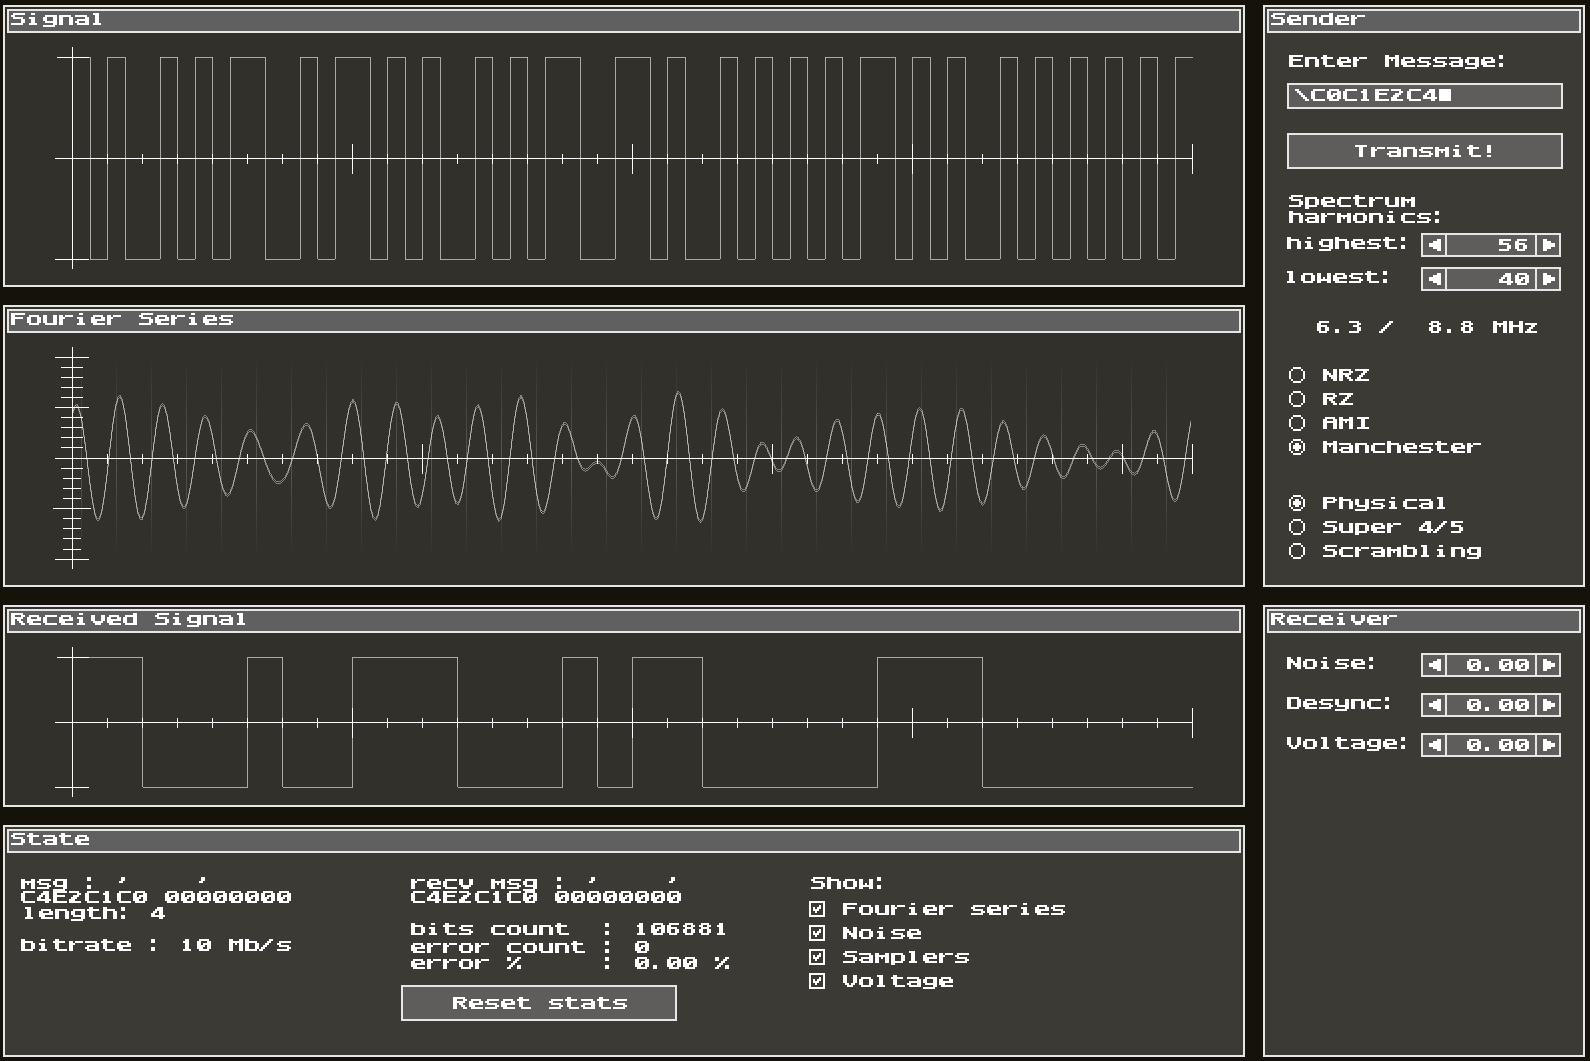
\includegraphics[width=0.95\linewidth]{./data/ideal_m2_min_f.png}
	\cutpic{0.2cm}{10cm}{./data/6_rz.png.jpg}
	\caption{F =  2.5 - 12.2 Мгц}
    \vspace{-1.7cm}
\end{wrapfigure}

\vspace{0.5cm}
Для метода RZ требуемая ширина полосы пропускания реального канала связи составила 9.7 МГц.
Для передачи данных без ошибок в реальном канале связи пришлось увеличить верхнюю границу на 3.4 МГц, а нижнюю уменьшить на 1.6 Мгц. Ширина полосы пропускания увеличилась с 4.7 МГц до 9.7 МГц (изменилась на +5 МГц). Это было необходимо для преодоления средних уровней помех, которые оказались выше, чем максимально допустимые уровни, рассчи-\\танные для данного метода на этапе 3.

\thispagestyle{empty}


\subsection{M2}

Для метода M2 требуемая ширина полосы пропускания реального канала связи составила 3.1 МГц.
Для передачи данных без ошибок в условия реального канала связи пришлось увеличить верхнюю границу на 0.6 МГц. Ширина полосы пропускания увеличилась с 2.5 МГц до 3.1 МГц (изменилась на +0.6 МГц). Это было необходимо для преодоления средних уровней помех.

\vspace{0.4cm}
\begin{figure}[H]
	\centering
	% 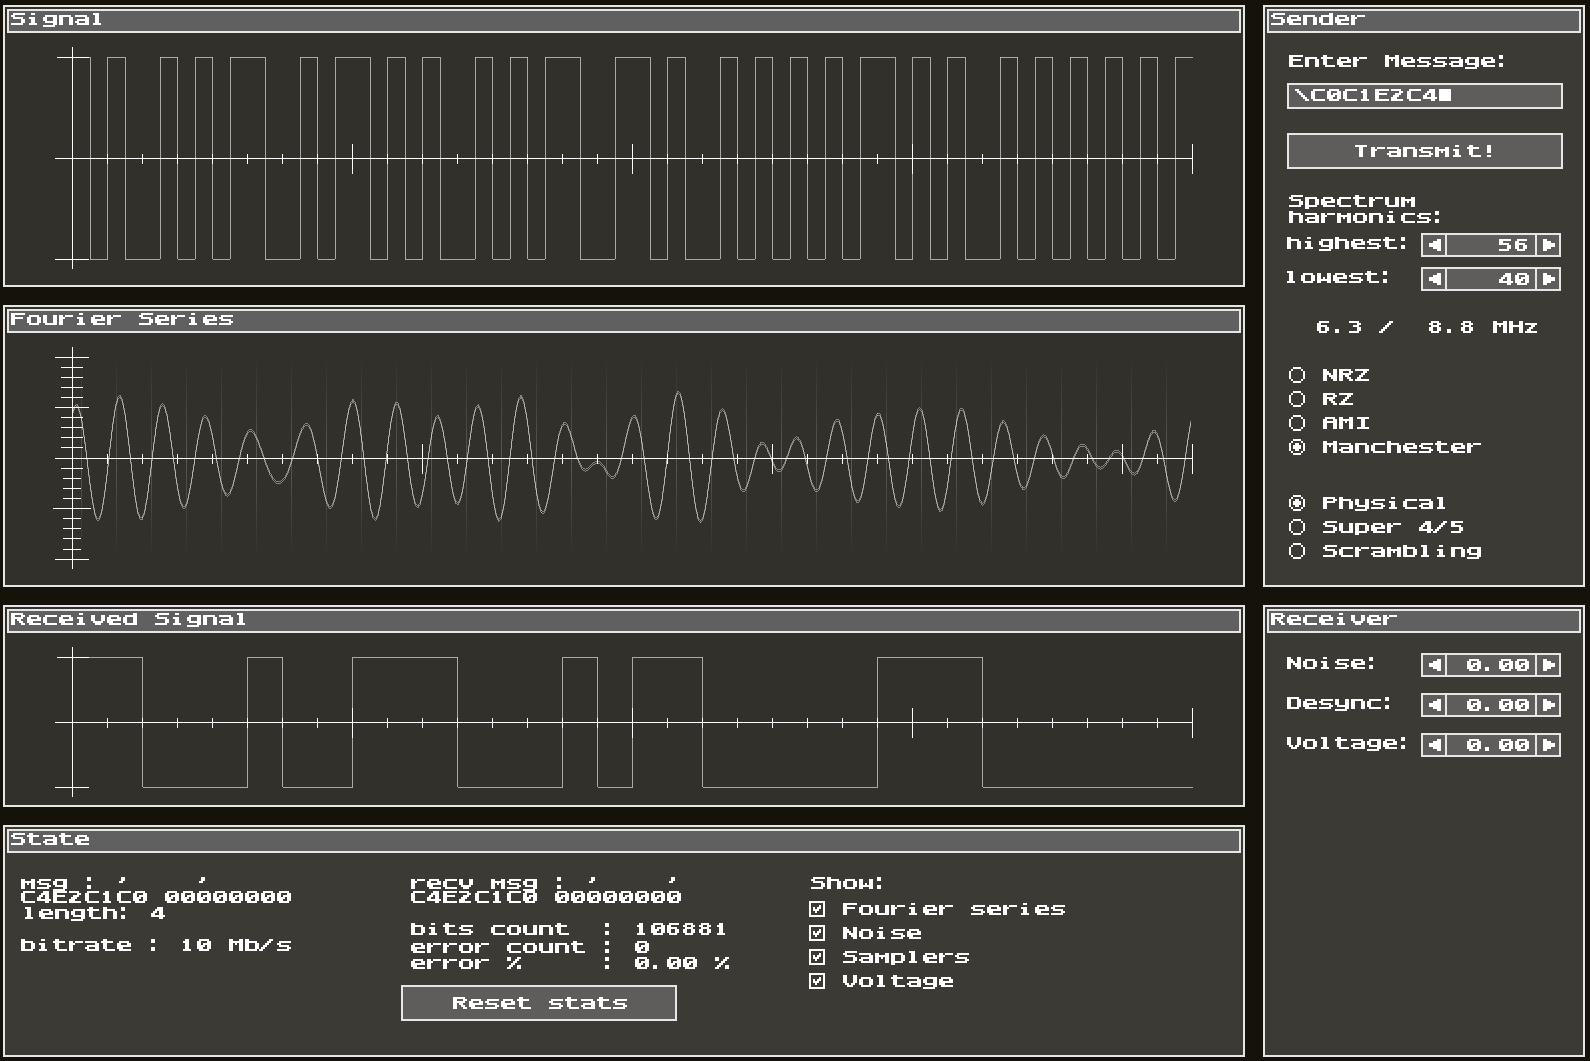
\includegraphics[width=0.95\linewidth]{./data/ideal_m2_min_f.png}
	\cutpic{0.2cm}{17.2cm}{./data/6_m2.png.jpg}
	\caption{F =  6.3 - 9.4 Мгц}
\end{figure}

\vspace{1.5cm}
\subsection{NRZ + 4B/5B}

Для метода NRZ+4B/5B требуемая ширина полосы пропускания реального канала связи составила 5.7 МГц.
Для передачи данных без ошибок в условия реального канала связи пришлось увеличить верхнюю границу на 1.5 МГц, а нижнюю уменьшить на 1.7 Мгц. Ширина полосы пропускания увеличилась с .2.5 МГц до 5.7 МГц (изменилась на +3.2 МГц). Это было необходимо для преодоления средних уровней помех, которые оказались сильно выше, чем максимально допустимые уровни, рассчитанные для данного метода на этапе 3.

\vspace{0.4cm}
\begin{figure}[H]
	\centering
	% 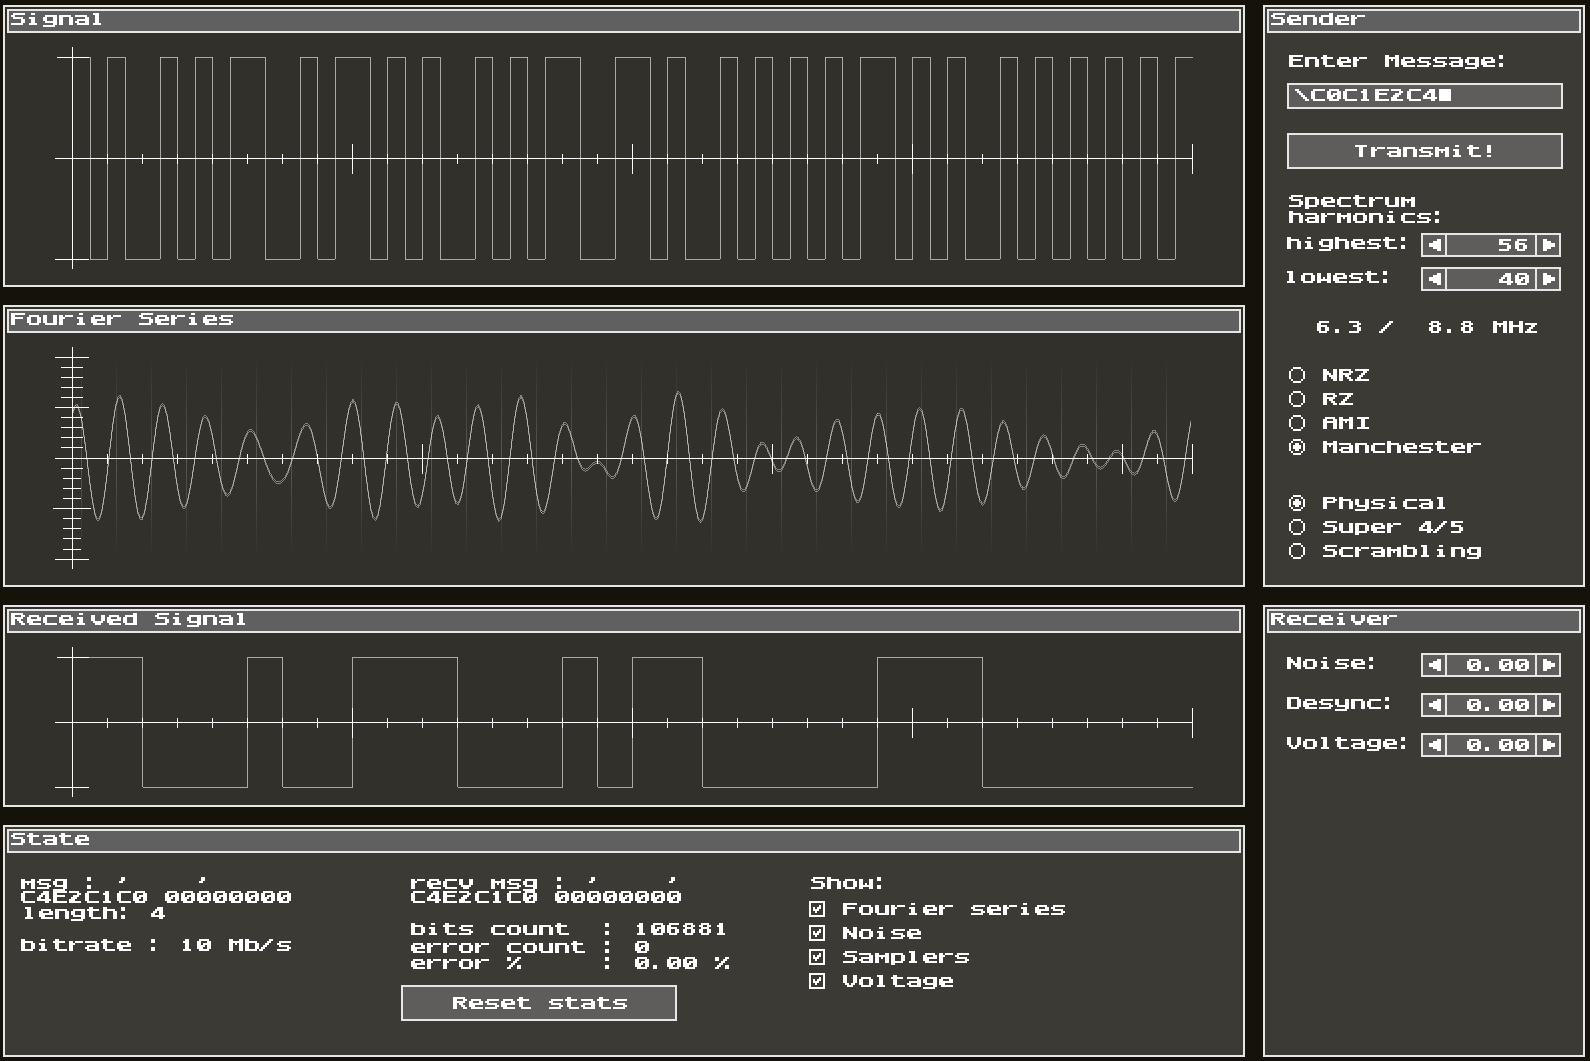
\includegraphics[width=0.95\linewidth]{./data/ideal_m2_min_f.png}
	\cutpic{0.2cm}{17.2cm}{./data/6_nrz45.png.jpg}
	\caption{F =  6.3 - 9.4 Мгц}
\end{figure}

\subsection{NRZ + Scramble}

Для метода NRZ+Scramble требуемая ширина полосы пропускания реального канала связи составила 4.4 МГц.

\vspace{0.4cm}
\begin{wrapfigure}{r}{0.6\textwidth}
	\centering
	% 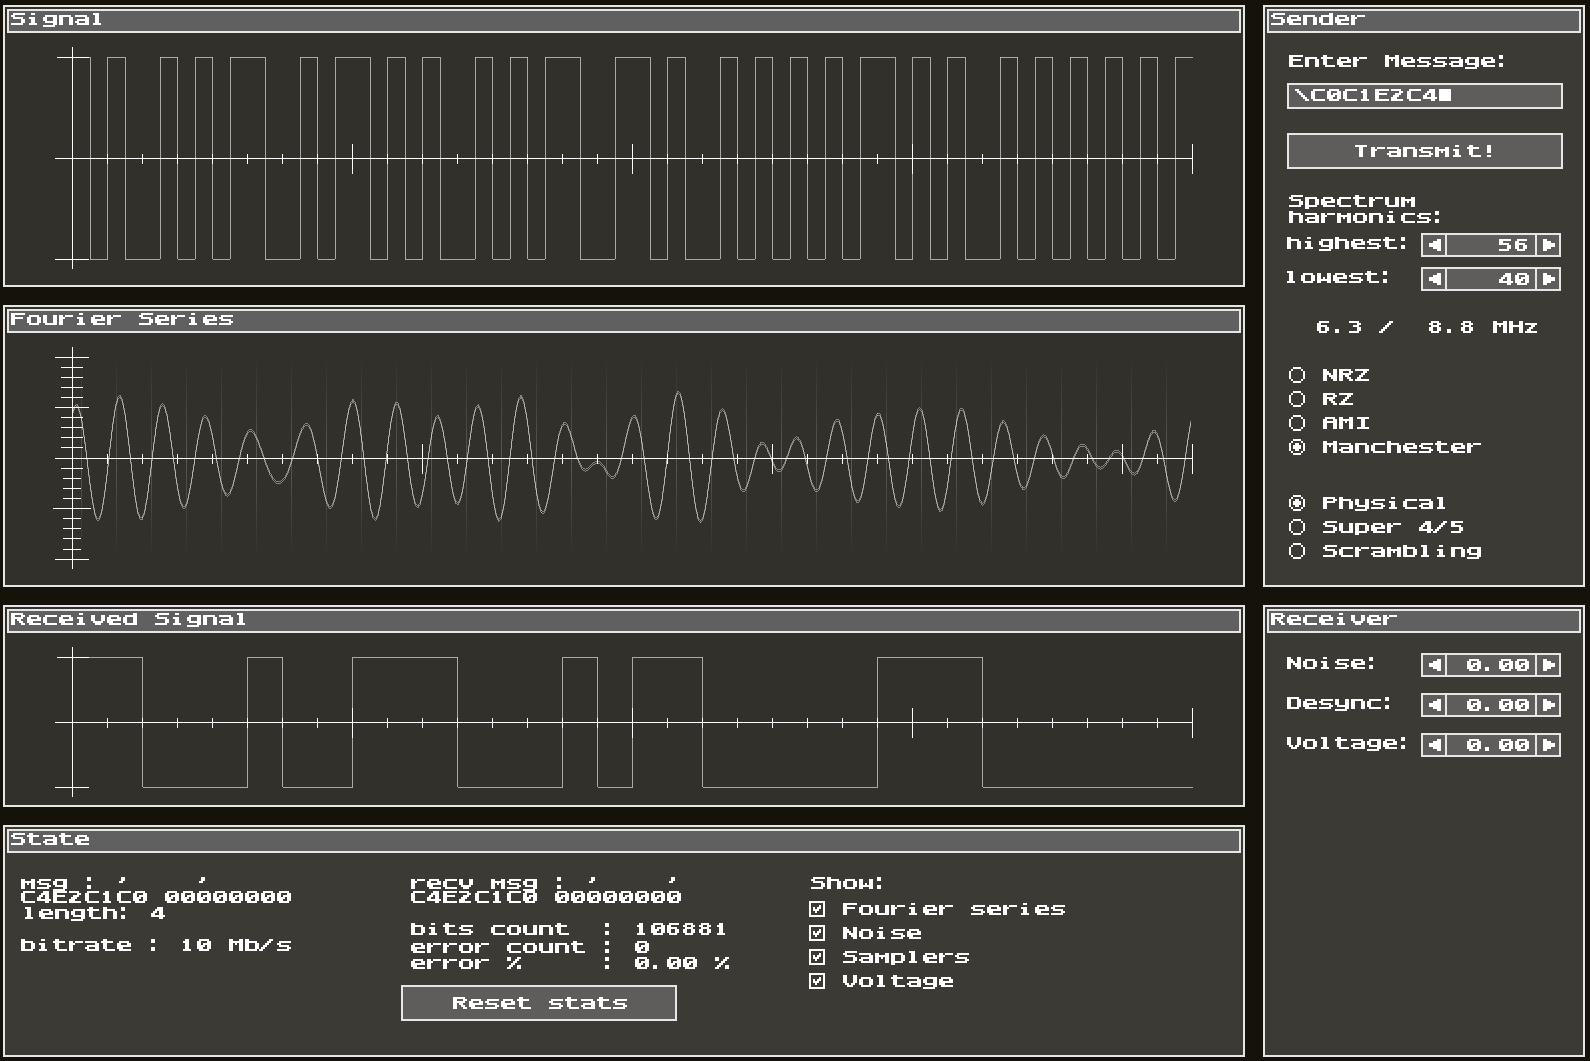
\includegraphics[width=0.95\linewidth]{./data/ideal_m2_min_f.png}
	\cutpic{0.2cm}{11.6cm}{./data/6_nrzS.png.jpg}
	\caption{F =  6.3 - 9.4 Мгц}
	\vspace{-1.7cm}
\end{wrapfigure}

Для передачи данных без ошибок в условия реального канала связи пришлось уменьшить нижнюю границу на 0.3 Мгц. Ширина полосы пропускания увеличилась с .4.1 МГц до 4.4 МГц (изменилась на +0.3 МГц). Это было необходимо для преодоления средних уровней помех, которые оказались выше, чем максимально допустимые уровни, рассчитанные для данного метода на этапе 3.

\subsection{Выводы}

Так как на третьем этапе NRZ и M2 показали наибольшие допустимые уровни помех, то при применении к ним уже средних уровней помех, их полоса пропускания не показала значительных изменений. \underline{Эти методы дали лучший} \underline{результат в \textbf{3.1 МГц}}.

На третьем этапе худшую устойчивость к помехам показали RZ и NRZ+4B/5B, поэтому при среднем уровне помех у них также худший результат по полосе пропускания – 9.7 и 5.7 МГц соответственно.

На третьем этапе NRZ+Scramble дал средний результат, поэтому при среднем уровне помех у него также средняя полоса пропускания (4.4 МГц).

